% adding the line below for Multifile document support with LatexTools Sublime package 
%!TEX root = manuscript.tex
\documentclass[12pt,a4paper,english]{article}


\usepackage[utf8]{inputenc}
\usepackage[english]{babel}

% Quotes 
\usepackage[square]{natbib}
\bibliographystyle{abbrvnat}

% For hyperlinks in the pdf 
\usepackage{hyperref}

% Glossaries
\usepackage[acronym]{glossaries}

% Font Helvetica
\renewcommand{\familydefault}{\sfdefault}
\usepackage[T1]{fontenc}

% Margins
%\usepackage[hmarginratio=2:2,top=25mm,columnsep=30pt]{geometry}
\usepackage{geometry}
 \geometry{
 a4paper,
 total={170mm,257mm},
 left=20mm,
 top=20mm,
 }
\linespread{1.5}

% For pictures in the pdf
\usepackage{graphicx}

% For tables
\usepackage{multirow}
\usepackage{booktabs}
\usepackage{threeparttable}

% For ref with figure, table or equation before the number
\usepackage{cleveref}

% landscape page
\usepackage{lscape}

% for argmin and argmax
\usepackage{amsmath}
\DeclareMathOperator*{\argmin}{argmin}

% for guillemets
\usepackage[T1]{fontenc}



% This is for me to comment

% Not using the pdfcomment package but it is an interesting one  
%\usepackage[author={Louis Mayaud}]{pdfcomment}

% Select what to do with todonotes: 
% \usepackage[disable]{todonotes} % notes not showed
\usepackage[draft]{todonotes}   % notes showed

% Select what to do with command \comment:  
% \newcommand{\comment}[1]{}  %comment not showed
\newcommand{\comment}[1]
{\par {\bfseries \color{blue} #1 \par}} %comment showed


\makeglossaries

\newacronym{adhd}{ADHD}{Attention Deficit/Hyperactivity Disorder}
\newacronym{nfb}{NFB}{neurofeedback}
\newacronym{eeg}{EEG}{electroencephalogram}
\newacronym{smr}{SMR}{Sensorimotor Rhythm}
\newacronym{mri}{MRI}{Magnetic Resonance Imagery}
\newacronym{tbr}{TBR}{Theta Beta Ratio}
\newacronym{scp}{SCP}{Slow Cortical Potential}
\newacronym{erp}{ERP}{Event-Related Potential}
\newacronym{rct}{RCT}{Randomized Controlled Trial}
\newacronym{hkd}{HKD}{Hyperkinetic Disorder}
\newacronym{es}{ES}{Effect Size}
\newacronym[plural=SEs, firstplural=Summary Effects]{se}{SE}{Summary Effect}
\newacronym{irb}{IRB}{Institutional Review Board}
\newacronym{ols}{OLS}{Ordinary Least Squares}
\newacronym{wls}{WLS}{Weighted Least Squares}
\newacronym{wrss}{WRSS}{Weighted Residual Sum of Squares}
\newacronym{lasso}{LASSO}{Least Absolute Shrinkage and Selection Operator}
\newacronym{pblind}{PBLIND}{Probably Blind}
\newacronym{mprox}{MPROX}{Most Proximal}
\newacronym{eog}{EOG}{Electro-Oculogram}
\newacronym{mse}{MSE}{Mean Square Error}
\newacronym{tova}{TOVA}{Test of Variables of Attention}
\newacronym{cpt}{CPT}{Continuous Performance Test}
\newacronym{sart}{SART}{Sustained Attention to Response Task}
\newacronym{fmri}{fMRI}{functional Magnetic Resonance Imaging}
\newacronym{pet}{PET}{Positron Emission Tomography}
\newacronym{saob}{SAOB}{Systematic Analysis of Biases}
\newacronym{agcl}{AgCl}{Silver Chloride}
\newacronym{au}{Au}{Gold}
\newacronym{emg}{EMG}{Electromyogram}
\newacronym{iapf}{iAPF}{individual Alpha Peak Frequency}


\begin{document}



\title{Supplemental material}
\date{}
\maketitle

\section{Materials and methods}

\subsection{Studies selection}
Search terms entered in Pubmed (last check on 14/12/2017) were: 
\guillemotleft ADHD OR adhd OR attention deficit disorder with hyperactivity OR minimal brain disorders OR syndrome hyperkinetic OR hyperkinetic
syndrome OR hyperactivity disorder OR hyperactive child syndrome OR childhood hyperkinetic syndrome OR attention deficit hyperactivity disorders
OR attention deficit hyperactivity disorder OR adhd attention deficit hyperactivity disorder OR addh OR overactive child syndrome OR attention deficit hyperkinetic 
disorder OR hyperkinetic disorder OR attention deficit disorder hyperactivity OR attention deficit disorders hyperactivity OR child attention deficit disorder 
OR hyperkinetic syndromes OR syndromes hyperkinetic OR hyperkinetic syndrome childhood) AND (randomized control trial OR RCT OR randomized control study OR Pilot
Study OR Study OR Trial OR randomized trial) AND (neurofeedback OR “EEG biofeedback” OR neurotherapy OR SCP OR “slow cortical potentials OR Theta Beta Ratio or TBR”\guillemotright.


\subsection{Perform a meta analysis}

To conduct meta-analysis, different software exist: for instance \citet{Cortese2016} used RevMan 5.3 \citep{RevMan} that computes the \gls{es} and its 
variance of each included study by applying the formula presented in \citet{Morris2008}. However, in order to compute the variance of the \gls{es}, 
the pooled within-group Pearson correlation $\rho$ (i.e the pre-post correlation) was required 
\citep{James2013}. In our case, this correlation was not known and the raw data were not available so we took an
 approximation: \citet{Balk2012} found that a value of 0.5 yields values closer to those computed with the right value of the correlation. 

In this replication of the work of \citeauthor{Cortese2016}, the same formulas are used \citep{Borenstein2009} but instead of using RevMan, 
a Python code was developed in order to perform the meta-analysis. To increase replicability and transparency and promote open science, we 
provide the full raw data used for this research as well as the Python code on a GitHub repository \citep{Bussalb2018}; it is tested
with \citet{Cortese2016} raw data to show that same results were found and could be used for replication and expansion of this work. The toolbox
could also be used to run any similar meta-analysis. 

To perform the meta-analysis several steps must be followed. First the choice of the model: this analysis is based on either one of the following 
statistical models \citep{Borenstein2009}:
\begin{itemize}
    \item \emph{the fixed-effect model}: the true \gls{es} (i.e the \gls{es} that would be observed with an infinitely 
		large sample size) is the same for all the studies in the analysis. The differences between the actually observed \gls{es}s 
		are due to sampling errors;
    \item \emph{the random-effects model}: the true \gls{es} could vary from study to study. The differences between the observed
		\glspl{es} are due to sampling errors but also to the various designs of the studies (for instance the number of participants or the implementation).
\end{itemize}

In the present case, although the studies included into the meta-analysis meet the same criteria, they remain different from each other 
on various points, so the random effects model is more appropriate than the fixed-effect model.  

\subsection{Compute the effect size of each study}

First, the scores presented in the articles were extracted and the \gls{es} of each study as defined in \citet{Morris2008} 
was computed 

\begin{equation}
\label{eq:metareview_effect_size}
\text{ES} = c_p \left[ \frac{(M_{\text{post},T} - M_{\text{pre},T}) - (M_{\text{post},C} - M_{\text{pre},C}) }{\sigma_{\text{pre}}} \right ].
\end{equation} 
An \gls{es} is exactly equivalent to a z-score of a standard normal distribution, it is computed as mean pre- to post-treatment 
score change in the \gls{nfb} group ($M_{\text{pre},T}$, $M_{\text{post},T}$) minus the mean pre- to post- treatment score change 
in the control group ($M_{\text{pre},C}$, $M_{\text{post},C}$), divided by the pooled pre-test standard deviation ($\sigma_{\text{pre}}$) 

\begin{equation}
\label{eq:stats_metareview_std_pre}
\sigma_{\text{pre}} = \sqrt{\frac{(n_T - 1)\sigma_{\text{pre},T}^2 + (n_C - 1)\sigma_{\text{pre},C}^2} {n_T + n_C - 2}},
\end{equation}

where $\sigma_{t,G}$ indicates the standard deviation for group $G$ at time $t$ and $n_G$ defines the sample size of each group; 
$c_p$ is a bias adjustment typically used for small sample sizes

\begin{equation}
\label{eq:metareview_correction_factor}
c_p =  1 - \frac{3} {4(n_T + n_C - 2) - 1}. 
\end{equation} 

\subsection{Compute the variance of each effect size}

Then, the variance of each \gls{es} was computed \citep{Morris2008}
\begin{equation}
\label{eq:metareview_variance_ES}
\sigma^2(\text{ES}) = c_p^2 \left (\frac{n_T + n_C - 2} {n_T + n_C - 4} \right ) \left  [ \frac{2(1-\rho)(n_T + n_C)} {n_Tn_C} + \text{ES}^2 \right ] - \text{ES}^2.
\end{equation} 

To compute the variance of the \gls{es}, the pooled within-group Pearson correlation $\rho$ (i.e the pre-post correlation) was required 
\citep{James2013}:

\begin{equation}
\label{eq:metareview_within_group_pearson_correlation}
\rho =  \frac{ \sum_{i=1}^{n} (\text{pre}_i - \mu_{\text{pre}})(\text{post}_i - \mu_{\text{post}}) } { \sqrt{ \sum_{i=1}^{n} (\text{pre}_i - \mu_{\text{pre}})^2} \sqrt{\sum_{i=1}^{n} (\text{post}_i - \mu_{\text{post}})^2} }, 
\end{equation}
where $n$ is the number of patients included in a study, $pre_i$, $post_i$ are score values for patient $i$ at pre- and post-test 
respectively, and $\mu_{pre}$, $\mu_{post}$ the mean scores over all patients. It is a measure of linear correlation between two variables. 
A value of 1 means that there is a positive correlation whereas a value of -1 means a negative correlation. When $\rho=0$, there is no
linear correlation. In our case, this correlation was not known and the raw data were not available so we took an
approximation: \citet{Balk2012} found that a value of 0.5 yields values close to those computed with the right value of the correlation. 

Once variances were obtained with \cref{eq:metareview_variance_ES}, we could compute the standard error and the 95\% confidence interval of each \gls{es}. 

\subsection{Compute the weight of each study}

To compute the \gls{se} a weight must be assigned to each study. To obtain them several steps must be followed. At first, the fixed-effects model 
weight $w_{fixed}$ of each study $k$ was computed as defined in \citet{Borenstein2009}: 

\begin{equation}
\label{eq:metareview_weight_fixed_study}
w_{\text{fixed}_k} = \frac{1}{\sigma^2(\text{ES}_k)}.
\end{equation} 

Nevertheless, we chose to use the random effects model, so the weights associated to this model are different. To compute them, the between-studies 
variance $\tau^2$ is required. It was calculated in three steps described in \cref{eq:metareview_Q}, \cref{eq:metareview_C} and \cref{eq:metareview_Tau} 
\citep{Borenstein2009}:

\begin{equation}
\label{eq:metareview_Q}
Q = \sum_{k=1}^{K} (w_{\text{fixed}_k} \text{ES}_k^2),
\end{equation}

\begin{equation}
\label{eq:metareview_C}
C = \sum_{k=1}^{K} (w_{\text{fixed}_k} - \frac{ \sum_{k=1}^{K} (w_{\text{fixed}_k})^2 } { \sum_{k=1}^{K} (w_{\text{fixed}_k}) },
\end{equation}
with $K$ the total number of included studies.

\begin{equation}
\label{eq:metareview_Tau}
\tau^2 = \frac{Q - \text{df}}{C},
\end{equation}
with $\text{df} = K - 1$ the degrees of freedom.

The random-effects model takes into account the differences between the studies, so the weights are equal to the inverse of the addition between the 
within-study variance (the variance of the \gls{es}) and the between-studies variance

\begin{equation}
\label{eq:metareview_weight_study}
w_k = \frac{1}{\sigma^2(\text{ES}_k) + \tau^2}.
\end{equation} 

\subsection{Compute the summary effect}

Eventually, the weighted average of the $K$ \gls{es} was computed to obtain the \gls{se} as described in 
\cref{eq:metareview_summary_effect} \citep{Borenstein2009}:

\begin{equation}
\label{eq:metareview_summary_effect}
\text{SE} = \frac{\sum_{k=1}^{K} w_k \text{ES}_k} {\sum_{k=1}^{K} w_k}.
\end{equation} 

Once the \gls{se}  is obtained, we can compute its variance, its standard error, its 95\% confidence interval, its p-value, 
and $I^2$ estimating effects size's between studies heterogeneity. 

\subsection{Scales used for the meta-analysis}

All scales used for the meta-analysis are summarized here in order to facilitate the replication of this work.

\begin{table}[h!]
  \centering
  \caption{Clinical scales used to update \citet{Cortese2016} with our choices and the two new articles.}
% table clinical scales


\scriptsize
\begin{tabular}{l*{4}{c}r}
\centering
\textbf{Study} & \textbf{Outcome} & \textbf{Score Names - Parents ratings} & \textbf{Score Names - Teachers ratings} \\
\toprule
\multirow{3}{*}{ \cite{Arnold2014} } & Total & SNAP IV & SNAP IV \\
& Inattention & SNAP IV & SNAP IV \\
& Hyperactivity & SNAP IV & SNAP IV \\
\midrule
\multirow{3}{*} { \cite{Bakhshayesh2011} } & Total & German ADHD-RS & German ADHD-RS \\
& Inattention & German ADHD-RS & German ADHD-RS \\
& Hyperactivity & German ADHD-RS & German ADHD-RS \\
\midrule
\multirow{2}{*} { \cite{Baumeister2016} } & Total & DISYPS & - \\[2ex]
\midrule
\multirow{3}{*} { \cite{Beauregard2006} } & Total & CPRS & - \\
& Inattention & CPRS & - \\
& Hyperactivity & CPRS & - \\
\midrule
\multirow{3}{*} { \cite{Bink2014} } & Total & ADHD-RS self report & - \\
& Inattention & ADHD-RS self report & - \\
& Hyperactivity & ADHD-RS self report & - \\
\midrule
\multirow{2}{*} { \cite{Christiansen2014} } & Total & Conners-3 Parents & Conners-3 Teachers \\[2ex]
\midrule
\multirow{3}{*} { \cite{Gevensleben2009} } & Total & German ADHD-RS & German ADHD-RS \\
& Inattention & German ADHD-RS & German ADHD-RS \\
& Hyperactivity & German ADHD-RS & German ADHD-RS \\
\midrule
\multirow{1}{*} { \cite{Heinrich2004} } & Total & German ADHD-RS & - \\[2ex]
\midrule
\multirow{3}{*} { \cite{Holtmann2009} } & Total & German ADHD-RS & - \\
& Inattention & German ADHD-RS & - \\
& Hyperactivity & German ADHD-RS & - \\
\midrule
\multirow{2}{*} { \cite{Linden1996} } & Total & IOWA Conners & - \\
& Inattention & IOWA Conners & - \\
\midrule
\multirow{3}{*} { \cite{Maurizio2014} } & Total & CPRS & CTRS \\
& Inattention & CPRS & CTRS \\
& Hyperactivity & CPRS & CTRS \\
\midrule
\multirow{3}{*} { \cite{Steiner2011} } & Total & Conners Rating Scales Revised & Conners Rating Scales Revised \\
& Inattention & Conners Rating Scales Revised & Conners Rating Scales Revised \\
& Hyperactivity & Conners Rating Scales Revised & Conners Rating Scales Revised\\
\midrule
\multirow{3}{*} { \cite{Steiner2014} } & Total & Conners-3 Parents & Conners-3 Teachers \\
& Inattention & Conners-3 Parents & Conners-3 Teachers \\
& Hyperactivity & Conners-3 Parents & Conners-3 Teachers\\
\midrule
\multirow{3}{*} { \cite{Strehl2017} } & Total & German ADHD-RS & German ADHD-RS \\
& Inattention & German ADHD-RS  & German ADHD-RS \\
& Hyperactivity & German ADHD-RS & German ADHD-RS \\
\midrule
\multirow{3}{*} {\cite{VanDongen2013} } & Total & ADHD RS & ADHD RS \\
& Inattention & ADHD RS & ADHD RS \\
& Hyperactivity & ADHD RS & ADHD RS \\
\bottomrule
\end{tabular}
\footnotesize
\centering
SNAP: Wanson, Nolan and Pelham Questionnaire, ADHD-RS: ADHD Rating Scale, CPRS: Conners Parent Rating Scale, CTRS: Conners Teacher Rating Scale, BOSS Classroom Observation: Behavioral Observation of Students in Schools, DISYPS: Diagnostic System of Mental Disorders in Children and Adolescents





  \label{Table:Table_mr_clinical_scales_update_cortese}
\end{table}


\subsection{Associate independent factors to effect sizes}

Three different methods were used to perform the \gls{saob}:
\begin{itemize}
	\item weighted multiple linear regression (\gls{wls}) \citep{Montgomery2012}; 
	\item sparsity-regularized linear regression with \gls{lasso} \citep{Tibshirani1996};
	\item decision tree \citep{Quinlan1986}.
\end{itemize}

We first applied the \gls{wls} as described in \cref{eq:factors_model_WLS}: 

\begin{equation}
\label{eq:factors_model_WLS}
\textbf{W}y = \textbf{WX}\beta + \epsilon.
\end{equation}

$\textbf{X}$ is a $(n \times p)$ full rank matrix and represents $n$ observations on each $p-1$ independent variables and an 
intercept term, $\beta$ is a $(p \times 1)$ vector of associated regression coefficients, $\textbf{W}$ is a $(n \times n)$ diagonal 
matrix with weights, $y$ is a $(n \times 1)$ vector of dependent variables and $\epsilon$ is a $(n \times 1)$ vector of errors.

The aim of the \gls{wls} is to estimate the vector of coefficients $\beta$ by minimizing the \gls{wrss}

\begin{equation}
\label{eq:factors_WRSS}
\text{WRSS} = \sum_{i=1}^{n} w_i \Big(y_i - \beta_{0} - \sum_{j=1}^{p}\beta_{j}x_{ij}\Big)^2.
\end{equation}

A significant coefficient (meaning significantly different from 0) indicates that the associated factor had probably an influence on \gls{nfb} efficacy and the sign 
of the coefficient indicates the direction of the effect.

The second method applied was the \gls{lasso} that naturally incorporates variable selection 
in the linear model thanks to $\ell-1$-norm applied on the coefficients. The coefficients $\hat{\beta}_j$ are obtained by minimizing the term

\begin{equation}
\label{eq:factors_lasso-minimization}
\hat{\beta} = \argmin_\beta \sum_{i=1}^{n} \Big(y_i - \beta_{0} - \sum_{j=1}^{p}\beta_{j}x_{ij}\Big)^2 + \lambda \sum_{j=1}^{p}|\beta_{j}|,
\end{equation} 

where $\lambda$ is the regularization parameter setting more coefficients to zero as it increases. The optimal tuning parameter was determined 
by a leave-one-out cross-validation. This method retains 1 observation as the validation data for testing the model and the 
remaining $n$ - 1 observations are used as training data. The cross-validation process is then repeated $n$ times with each of the observation 
used exactly once as the testing data. For each fold, the \gls{mse} on the test set was computed and eventually, the $n$ results can 
be averaged to produce a single observation that enables to find the optimal $\lambda$: it corresponds to the abscissa of the minimum
value of the \gls{mse} on the mean fold computed for a large range of $\lambda$ \citep{James2013}. 
A coefficient not set at zero means that the associated factor may have an influence on \gls{nfb} and once again,
the sign of the coefficient indicates the direction of the effect.

Eventually, the last method used to determine factors influencing \gls{nfb} was the decision tree \citep{Quinlan1986}, a non linear method. It brakes down a dataset into smaller
and smaller subsets using at each iteration a variable and a threshold chosen to optimize a simple \gls{mse} criteria 

\begin{equation}
\label{eq:factors_decision_tree_mse}
\text{MSE} = \frac{1}{n}\sum_{i=1}^{n} \Big(\hat{y}_i - {y}_i\Big)^2,
\end{equation}

with $\hat{y}$ the predicted values.

No weights are applied when running the \gls{lasso} and the decision tree because the frameworks don't easily account for this.


\clearpage

\section{Results}

\subsection{Perform a meta-analysis}

First, when using the \gls{es} found by \citet{Cortese2016} thanks to RevMan \citep{RevMan}, and then performed the following steps 
of meta-analysis with the Python code, we observe no major differences between these results and those obtained with RevMan \citep{RevMan} 
as listed in \cref{Table:meta_review_comparison_between_revman_python}. The minor discrepancies, especially observed at the p-values level,
are due to our choice to always use a pre-post correlation of 0.5 when computing the variance of each \gls{es}. Moreover, a sensitivity 
analysis was conducted to ensure the minor impact of the pre-post correlation value: when it varies between 0.2 and 0.8 the significance 
of the \gls{se} does not change. 

\begin{table}[h!]
  \centering
  \caption{Comparison between \citet{Cortese2016} results obtained with RevMan \citep{RevMan} and those obtained with the Python code. Summary 
	effects and their corresponding p-value in parenthesis are presented. With the Python program, a negative summary effect is in favor of \gls{nfb}.}
\begin{tabular}{ |p{2cm}|p{2.5cm}|p{4cm}|p{4.5cm}|  }
\hline
 \multicolumn{2}{ |c| }{Input data} & Results from \citet{Cortese2016} & Effect sizes from \citet{Cortese2016}\\
\hline
\multicolumn{2}{ |c| }{Implementation} & RevMan \citet{RevMan} & Python program\\
\hline
\multirow{3}{*}{ \textit{Parents} } & Total & $0.35$ ($0.004$) & $-0.34$ ($0.004$)\\
 & Inattention  & $0.36$ ($0.009$) & $-0.35$ ($0.011$)\\
 & Hyperactivity  & $0.26$ ($0.004$) & $-0.24$ ($0.02$)\\
\hline
\multirow{3}{*}{ \textit{Teachers} } & Total & $0.15$ ($0.20$) & $-0.13$ ($0.25$)\\
 & Inattention  & $0.06$ ($0.70$) & $-0.09$ ($0.50$)\\
 & Hyperactivity  & $0.17$ ($0.13$) & $-0.15$ ($0.21$)\\
 \hline
\end{tabular}

  \label{Table:meta_review_comparison_between_revman_python}
\end{table}

Thanks to the previous step, we can conclude that the Python code yields results close to those returned by RevMan \citet{RevMan}, so we decide to
use this code to perform our meta-analysis.		

\subsection{Detect factors influencing the Neurofeedback}
		
To assess the variability of each factor, box plots of their standardized values were displayed in \cref{Figure:factors_analysis_boxplots}: treatment length, 
session length and number of sessions are more variable across studies than session pace, minimum and maximum age.  

\begin{figure}[h!]
	\center
  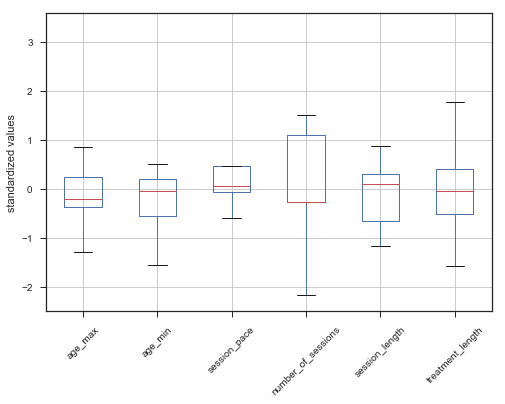
\includegraphics[scale=0.5]{figures/factors_analysis_boxplot_no_colors_no_two_columns}
  \caption{Boxplots of the standardized values of each continuous factor.}
  \label{Figure:factors_analysis_boxplots}
\end{figure}

\subsection{Assumptions for applying linear regression}

The first method used to detect the influencing factors was the \gls{wls}. The assumptions inherent to this method are checked: 
\begin{itemize}
	\item the moment matrix $\mathbf{{X}^{T}W^{T}WX}$ was invertible;
  \item no apparent correlation between the continuous independent variables was found; 
  \item the fit was significant as shown by the F-statistic (prob(F-statistic) = 2.81e-10); 
  \item the residuals were normally distributed as demonstrated by the skew (-0.15), kurtosis (2.81) and the Omnibus test (prob(Omnibus) = 0.87).
\end{itemize} 

These assumptions are also satisfied for the \gls{ols}.

\clearpage

\bibliography{bibliography}

\end{document}